\section{Resistência}

No capítulo anterior, fora apresentado que aplicar uma tensão através de um fio
ou circuito resulta em um fluxo de carga ou de corrente através do fio ou do
circuito. Entretando, por que a corrente é mai intensa em alguns circuitos que
em outros? O que determina o nível de corrente resultante de uma tensão em
particular? A resposta está no fato de que há uma oposição ao fluxo de carga no
sistema que depende dos componentes do circuito, sendo este chamado
\textit{resistência}, que tem unidades \textit{ohms} (\( \Omega \)).

Essa oposição, devido fundamentalmente a colisões e fricção entre os elétrons
livres e outros elétrons, íons e átomos no curso do movimento, converte a
energia elétrica fornecida em \textit{calor}. Estas interações termodinâmicas
dependem do material do resistor.

Assim podemos definir a resistência como:

\begin{equation}
	\label{eq:lei-de-ohm}
	R \overset{\triangle}{=} \rho \frac{l}{A}
\end{equation}

Sendo \textit{\( \rho \)} a resistividade do material e sendo medidas a CM-\(
\Omega \)/pés, \textit{l} sendo o comprimento do fio em pés e \textit{A} a área
da seção transversal ou em termos leigos a grossura do fio e é medido na unidade
CM.\@ Pode-se melhor visualizar tais grandezas na Figura~\ref{fig:fig4}.

\begin{figure}[H]
	\centering
	\setlength{\fboxsep}{0pt}
	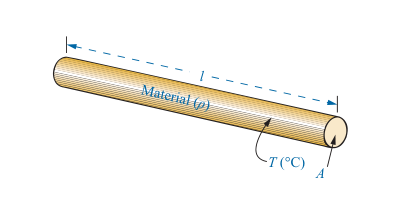
\includegraphics[height=0.15\textwidth]{./fig/fig4.png}
	\caption{Fatores que afetam a resistência de um condutor}
	\label{fig:fig4}
\end{figure}

% \[
% 	+\text{Potência absorvida} = –\text{Potência fornecida}
% \]
%
% \subsection{\textbf{Exemplos}}
%
% \begin{enumerate}
% 	\item Uma fonte de energia com uma corrente constante de 2 A força a passagem
% 	      dessa corrente através de uma lâmpada por 10 s. Se forem liberados 2,3 kJ
% 	      na forma de energia luminosa e calorífca, calcule a queda de tensão na
% 	      lâmpada.
% 	      \[
% 		      \begin{aligned}
% 			      \Delta q & = i \Delta t = 2 \cdot 10 = 20 \,\text{C}                          \\
% 			               & \hphantom{=} \text{A queda de tensão é}                            \\
% 			               & = \frac{\Delta w}{\Delta q} = \frac{2.3 \cdot 10^3}{20} \,\text{V} \\
% 			               & = 115 \,\text{V}                                                   \\
% 		      \end{aligned}
% 	      \]
% \end{enumerate}
